\section{Mortimer}\label{mortimer}


\begin{figure}
\centering

\includegraphics{Mortimer.png}
\caption{Mortimer.png}
\end{figure}

{[}Info generali{]}

Età: 12

Anno di nascita: 2011

Paese di nascita:

Razza: Goblin

Relazioni: Gilda dei Protettori

Alleati:

Nemesi:

Possedimenti importanti:


\subsection{Descrizione Generale}\label{descrizione-generale}


\begin{figure}
\centering
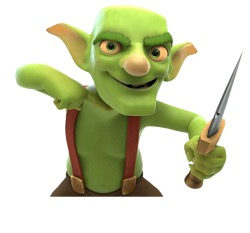
\includegraphics{Goblins_card_render.jpeg}
\caption{Goblins\_card\_render.jpeg}
\end{figure}

Un guerriero goblin con disturbo dell'attenzione.

\begin{quote}
``Voglio assaggiare quest'acqua di fogna''
\end{quote}

\subsection{Biografia}\label{biografia}


\begin{figure}
\centering

\includegraphics{2023-03-26_17.20.08.jpg}
\caption{2023-03-17.20.08.jpg}
\end{figure}

I genitori lo hanno mandato all'accademia militare con la speranza che
apprendesse disciplina e educazione, ma è scappato dopo un anno.

I genitori ancora lo cercano.

Per guadagnarsi da vivere ha scelto la strada più facile e sbagliata: il
crimine. Non ha legami con alcuna organizzazione in particolare,ma ha
dei contatti nella mala. Ogni tanto lo chiamano per dei lavori,
principalmente colpi a diligenze.

\subsection{Carriera}\label{carriera}


Nell'ultimo periodo si è affiliato alla Gilda dei Protettori della Sila
devoti a San Francesco e ai Lupi, un buon ``tetto sulla testa e una paga
decente'' a suo parere.

\subsection{Personalità}\label{personalituxe0}


Non ha ben in mente cosa sia bene e male, ma non perchè sia un goblin
(basta con gli stereotipi), viene da una famiglia per bene, gente che
gli ha dato un fior fiore di educazione\ldots{} Proprio è una testina di
cazzo.

